\section{Costruzione dello scheletro}
Vista la necessità di standardizzarsi sulle tecnologie e modalità in uso, la costruzione stessa dello scheletro 
ha seguito un approccio incrementale: si è iniziato da un microservizio, \textit{GestioneComanda}, per poi proseguire con \textit{GestioneCliente} e \textit{GestioneCucina}.

\subsection{Organizzazione del processo di sviluppo}
Per l’implementazione dei microservizi che compongono il sistema ServeEasy, attualmente delineato al primo zoom-in, è stato applicato un approccio “polyrepo"\cite{polyrepo}, definendo per ogni microservizio un’area di progetto dedicata. 

Scelta GitHub come piattaforma di hosting per il progetto software, un membro del team è stato incaricato del setup, controllo e gestione delle repository per i singoli microservizi.

Per raggiungere tale organizzazione, è stata prima di tutto creata un’area di lavoro per familiarizzare con le tecnologie selezionate, impiegando uno sforzo congiunto nello studio e prototipazione.

Nel processo di sviluppo sono state specificate delle regole mutualmente pattuite:
\begin{itemize}
    \item Nessuno esegue push diretto dall’area di lavoro locale verso il main branch: ognuno lavora esclusivamente sulla propria branch;
    \item Nei commit e nelle pull requests va espressa una sintesi del proprio lavoro svolto;
\item Cambiamenti importanti vanno discussi;
\item Ogni implementazione va testata;
\item Prima di effettuare una merge sul main branch, l’implementazione deve aver passato le fasi di build e di test con successo.
\end{itemize}

A supporto del processo di sviluppo, sono state introdotte automatizzazioni per garantire Continuous Integration e Continuous Delivery, servendosi di Github Workflows e Docker allo scopo di aumentare la velocità di deployment delle nuove modifiche apportate, garantendo al contempo integrità:
\begin{itemize}
    \item Un evento di push verso il proprio branch causa l’avvio della job di CI posta a sorveglianza del proprio spazio di lavoro sulla repository, allo scopo di effettuare un controllo di compilazione;
    \item Un evento verso il main branch (quale, ad esempio, una merge) causa l’avvio della job di CI/CD posta a sorveglianza del main sulla repository, la quale effettua un controllo di compilazione, genera un eseguibile e procede con le fasi di build e ship dell'immagine Docker corrispondente verso il registry DockerHub \cite{DockerOverview}.
\end{itemize}

In particolare, nel punto 2 si parla di Continuous Delivery e non Continuous Deployment, in quanto il deployment della nuova immagine va eseguita manualmente \cite{CDDocker}.

Il deployment verrà effettuato tramite Docker Compose: vengono definiti in un unico file i servizi offerti dal registry di riferimento (Dockerhub), le loro caratteristiche e dipendenze, cosicchè sarà sufficiente avviare il file per poter scaricare le immagini dei microservizi e servizi d’interesse in una rete di container dedicata.



\begin{figure}[htbp]
	\centering
	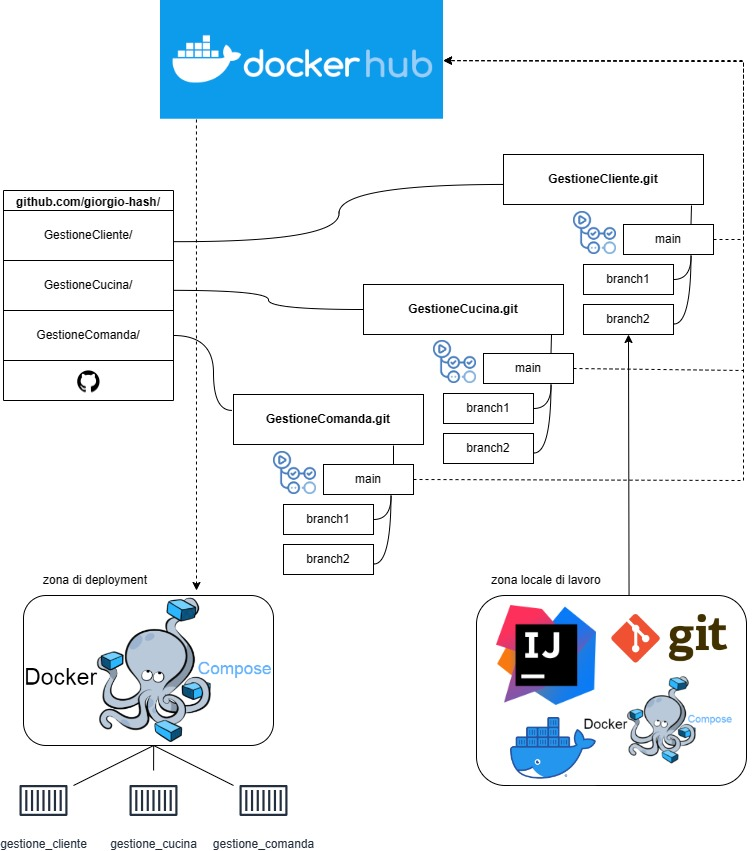
\includegraphics[scale=0.36]{iterazione1/images/DevOps.jpg}
	\caption{Organizzazione del lavoro cloud e locale, CI/CD e deployment 
 \label{fig:devopsit1}}
\end{figure}


\subsection{Organizzazione dell'area di lavoro}
Oltre all'IDE di Intellij IDEA e Git, l'area di lavoro locale è supportata da Docker Compose per attivare i servizi a supporto dell'esecuzione del singolo microservizio: non solo dipendenze, quali Kafka, Zookeeper ed il database MariaDB, ma anche strumenti utili per la visualizzazione ed interazione ad alto livello col sistema, quali:
\begin{itemize}
    \item Kafdrop per monitorare i messaggi passati tra pub e sub attraverso Kafka;
    \item PHPMyAdmin per monitorare, sviluppare ed iniettare dati nel database MariaDB.
\end{itemize}
Facendo leva sulla portabilità offerta dal framework Docker, viene garantito un ambiente altamente personalizzabile, flessibile e di facile implementazione. 

\begin{figure}[htbp]
	\centering
	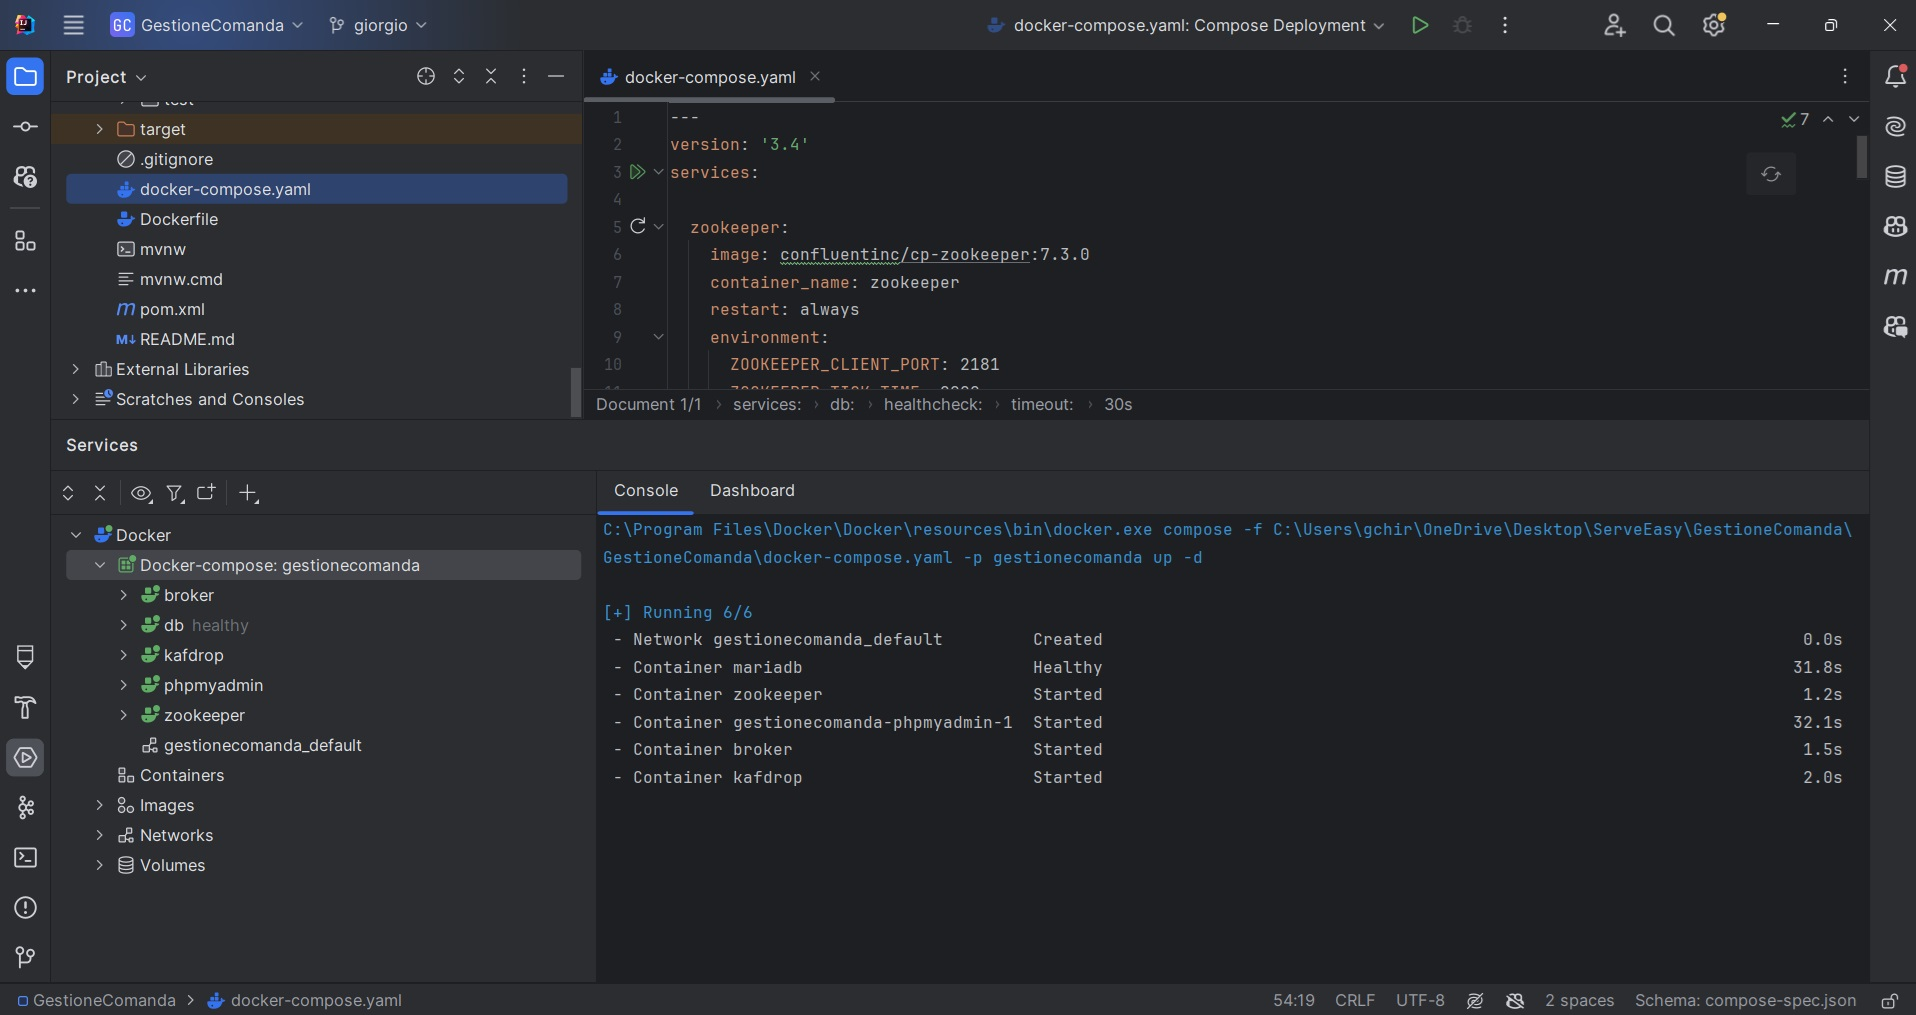
\includegraphics[scale=0.36]{iterazione1/images/IDEIDEA.jpg}
	\caption{Ambiente di lavoro con Intellij IDEA e Docker Compose
 \label{fig:IDEAit1}}
\end{figure}

\begin{figure}[htbp]
	\centering
	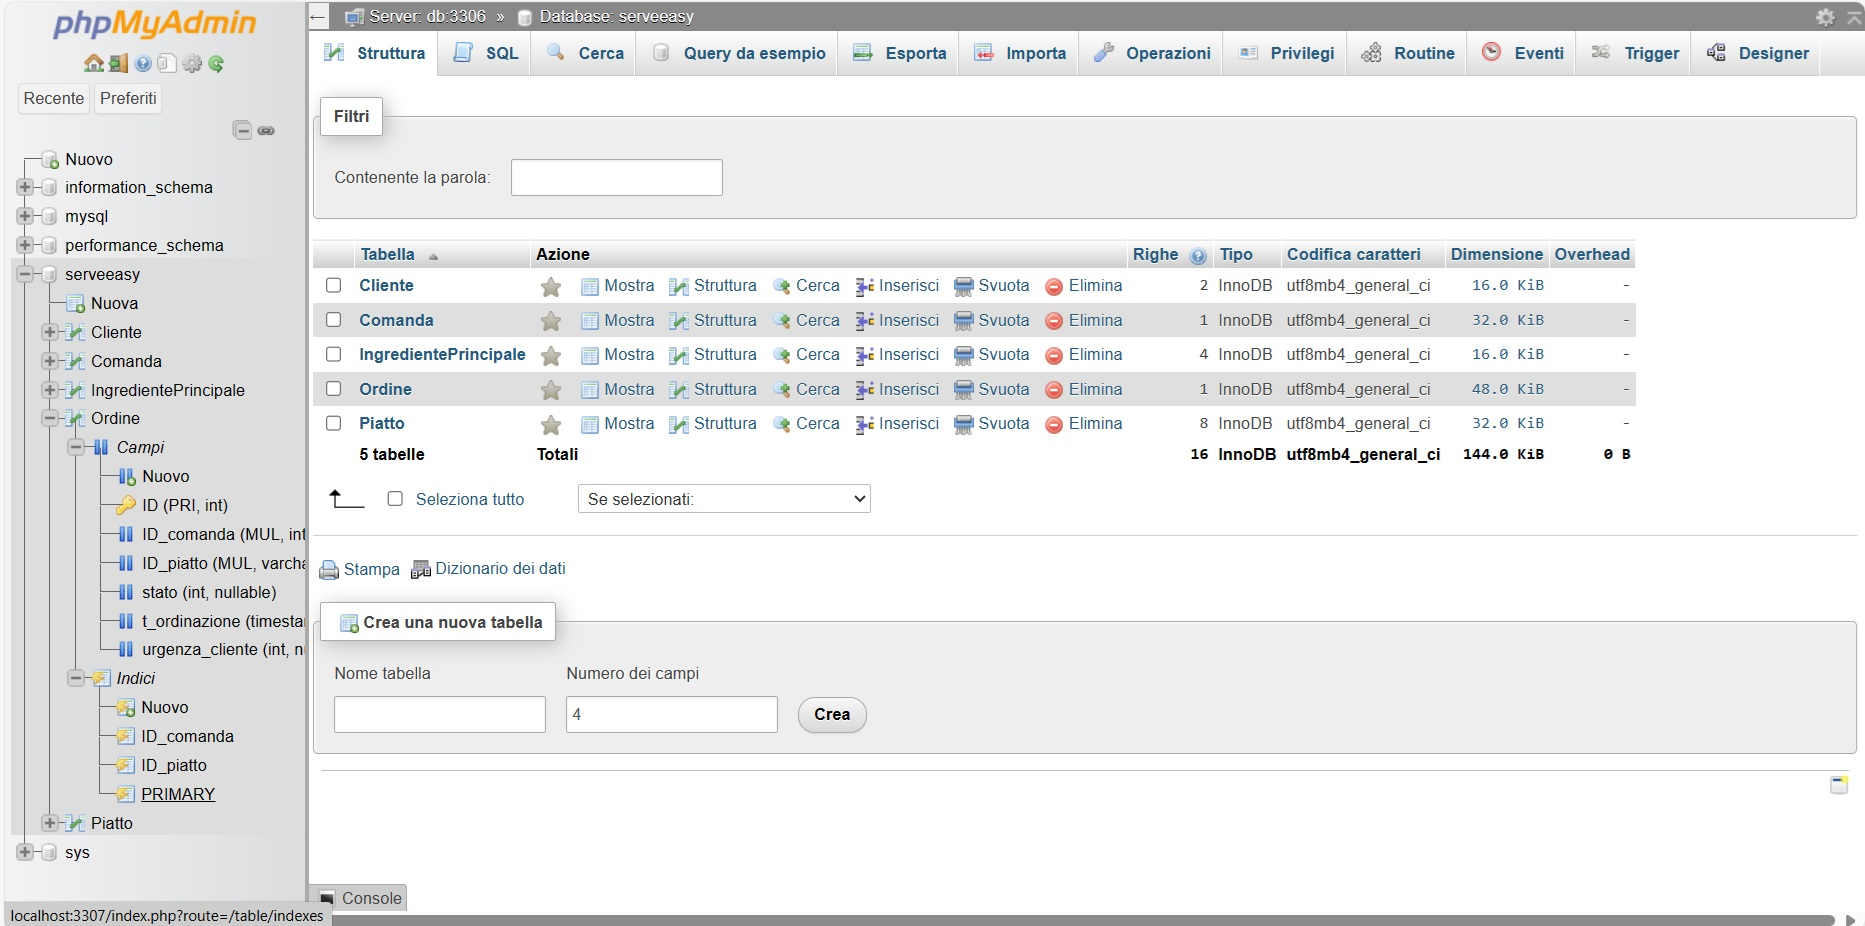
\includegraphics[scale=0.36]{iterazione1/images/phpmyadmin.jpg}
	\caption{interfaccia grafica di PHPMyAdmin eseguito da container
 \label{fig:phpmyadmin}}
\end{figure}


\subsection{Definizione Interfacce}
% nota: metterei solo quelle di gestione comanda oppure quelle che ci servono per spiegare
\begin{lstlisting}[style=myJava, 
    caption={Interfaccia MessagePort}, label=lst:messageport, emph={[3] send},
    emphstyle={[3]\color{codeCyan}}]
public interface MessagePort<T> {
    /**
     * Invia l'oggetto passato come parametro sul topic del message broker
     *
     * @param t oggetto da inviare
     * @throws JsonProcessingException eccezione sollevata nella serializzazione
     */
    void send(T t) throws JsonProcessingException;
}
\end{lstlisting}

\begin{lstlisting}[style=myJava, 
    caption={Interfaccia DataPort}, label=lst:dataport,
    emph={[3] isOrderExist, saveOrder, getOrderById, updateOrder, findAllOrdersByIdComanda, deleteOrder},
    emphstyle={[3]\color{codeCyan}}]
public interface DataPort {

    /**
     * Controlla se l'ordine esiste nel database
     *
     * @param id id dell'entita' ordine da controllare la presenza
     * @return true se esiste, false altrimenti
     */
    boolean isOrderExist(int id);

    /**
     * Salva l'entita' ordine all'interno del database
     *
     * @param ordineEntity entita' ordine da salvare
     * @return entita' ordine salvata
     */
    OrdineEntity saveOrder(OrdineEntity ordineEntity);

    /**
     * Cerca nel db e restituisce l'ordine corrispondente all' id dato
     *
     * @param id id dell'ordine
     * @return Optional(OrdineEntity) se esiste altrimenti Optional(null)
     */
    Optional<OrdineEntity> getOrderById(int id);

    /**
     * Aggiorna l'attributo stato dell'ordine
     *
     * @param id id dell'ordine su cui effetturare l'aggiornamento
     * @param ordineEntity entita' con gli aggiornamenti parziali da applicare
     * @return entita' aggiornata
     */
    OrdineEntity updateOrder(int id, OrdineEntity ordineEntity);


    /**
     * Lista di tutti gli ordini per una specifica comanda
     *
     * @param idComanda id della comanda su cui cercare gli ordini
     * @return lista di ordini per una data comanda
     */
    List<OrdineEntity> findAllOrdersByIdComanda(int idComanda);

    /**
     * Cancella l'ordine con il dato ID dal databse
     *
     * @param id id dell'ordine da eliminare
     */
    void deleteOrder(int id);
}
\end{lstlisting}

\begin{lstlisting}[style=myJava, 
    caption={Interfaccia NotifyOrderEvent}, label=lst:notifyordereventIF,
    emph={[3] getLastMessageReceived, receive},
    emphstyle={[3]\color{codeCyan}}]
public interface NotifyOrderEvent {

    /**
     * Riceve un messaggio tramite Kafka dal servizio gestioneCliente in merito all'avvenuta ordinazione
     * da parte di un cliente
     *
     * @param message il corpo del messaggio vero e proprio
     * @param topic topic del message broker sul quale si riceve il messaggio
     * @param partition numero di partizione sul quale si riceve il messaggio
     * @param offset numero di offset che presenta il messaggio ricevuto
     */
    @KafkaListener(id = "${spring.kafka.consumer.gestioneCliente.group-id}", topics = "${spring.kafka.consumer.gestioneCliente.topic}")
    void receive(String message, String topic, Integer partition, Long offset) throws JsonProcessingException;

    /**
     * Restituisce l'ultima notifica letta dal listener
     *
     * @return oggetto notifica letto dal listener
     */
    NotificaOrdineDTO getLastMessageReceived();
}
\end{lstlisting}

%TODO: ho aggiunto solo quelle che mi servono per poter avere il riferimento

\subsection{Adattatore Kafka}
Lo sviluppo del componente adibito all'adattatore Kafa è stato un processo che ha seguito vari step:
\paragraph{Step 1 - Overview:}
Come primo passo ci si è fatti una panoramica leggendo la documentazione ufficiale di Spring Kafka \cite{SpringKafka} e si sono cercati alcuni progetti su Github di \href{https://github.com/devtiro/spring-boot-kafka-tutorial/tree/main}{esempio}.
\paragraph{Step 2 - Setup:}
Al passo numero due ci si è focalizzati sul setup dell’ambiente di lavoro, si sono definiti i seguenti container nel file "docker-compose.yaml" (Codice \vref{lst:docker-compose1}):
\begin{lstlisting}[language=docker-compose, caption={Setup del docker-compose.yaml per l'adattatore Kafka}, label=lst:docker-compose1]
services:  
  zookeeper:
    image: confluentinc/cp-zookeeper:7.3.0
    container_name: zookeeper
    restart: always
    environment:
      ZOOKEEPER_CLIENT_PORT: 2181
      ZOOKEEPER_TICK_TIME: 2000

  broker:
    image: confluentinc/cp-kafka:7.3.0
    container_name: broker
    restart: always
    ports:
      - "9092:9092"
    depends_on:
      - zookeeper
    environment:
      KAFKA_BROKER_ID: 1
      KAFKA_ZOOKEEPER_CONNECT: 'zookeeper:2181'
      KAFKA_LISTENER_SECURITY_PROTOCOL_MAP: PLAINTEXT:PLAINTEXT,PLAINTEXT_INTERNAL:PLAINTEXT
      KAFKA_ADVERTISED_LISTENERS: PLAINTEXT://localhost:9092,PLAINTEXT_INTERNAL://broker:29092
      KAFKA_OFFSETS_TOPIC_REPLICATION_FACTOR: 1
      KAFKA_TRANSACTION_STATE_LOG_MIN_ISR: 1
      KAFKA_TRANSACTION_STATE_LOG_REPLICATION_FACTOR: 1
\end{lstlisting}
Fatto ciò si è passati ad aggiornare il file "pom.xml" (Codice \vref{lst:pom-xml1}) con la seguente dipendenza per Kafka: 
\begin{lstlisting}[language=XML, caption={Aggiornamento dipendenze nel pom.xml per includere spring-kafka}, label=lst:pom-xml1]
<dependency>
    <groupId>org.springframework.kafka</groupId>
    <artifactId>spring-kafka</artifactId>
</dependency>
\end{lstlisting}
Successivamente nel file "application.yml" (Codice \vref{lst:application-yml1}) sono state aggiunte le seguenti istruzioni di configurazione, come si può notare si è partiti inizialmente solamente a considerare un'applicazione costituita da un singolo producer senza consumer:
\begin{lstlisting}[language=yaml, caption={Aggiornamento del file `application.yml` per il producer Kafka}, label=lst:application-yml1]
spring:
  kafka:
    bootstrap-servers: localhost:9092
    producer:
      topic: sendOrderEvent
      group-id: gestioneComanda
\end{lstlisting}
Sono stati poi creati i primi bean di configurazione nella classe "KafkaConfig.java" (Codice \vref{lst:KafkaConfig}):
\begin{lstlisting}[style=myJava, 
    caption={Classe di configurazione KafkaConfig.java}, label=lst:KafkaConfig, 
    emph={[2] BOOTSTRAP_SERVERS_CONFIG, KEY_SERIALIZER_CLASS_CONFIG ,  VALUE_SERIALIZER_CLASS_CONFIG, bootstrapServers },
    emphstyle={[2]\color{codeDarkMagenta}},]
@Configuration
public class KafkaConfig {

    @Value("${spring.kafka.bootstrap-servers}")
    private String bootstrapServers;

    @Bean
    public ProducerFactory<String, String> producerFactory() {
        Map<String, Object> configProps = new HashMap<>();
        configProps.put(ProducerConfig.BOOTSTRAP_SERVERS_CONFIG, bootstrapServers);
        configProps.put(ProducerConfig.KEY_SERIALIZER_CLASS_CONFIG, StringSerializer.class);
        configProps.put(ProducerConfig.VALUE_SERIALIZER_CLASS_CONFIG, StringSerializer.class);
        return new DefaultKafkaProducerFactory<>(configProps);
    }

    @Bean
    public KafkaTemplate<String, String> kafkaTemplate() {
        return new KafkaTemplate<>(producerFactory());
    }
}
\end{lstlisting}
E di Object Mapper (Codice \vref{lst:jsonconfig}) per la serializzazione e deserializzazione in formato JSON, visto che la comunicazione tramite message broker avviene tramite messaggi in quel formato:
\begin{lstlisting}[style=myJava, 
    caption={Classe di configurazione JsonConfig.java}, label=lst:jsonconfig,]
@Configuration
public class JsonConfig {

    @Bean
    public ObjectMapper objectMapper(){
        final ObjectMapper objectMapper = new ObjectMapper();
        // configurazione di timestamp
        objectMapper.registerModule(new JavaTimeModule());
        objectMapper.setDateFormat(new SimpleDateFormat("yyyy-MM-dd HH:mm:ss.SSS"));
        return objectMapper;
    }
}
\end{lstlisting}
\paragraph{Step 3 - Producer:}
Nel passo successivo si è passati a creare la prima classe adibita al compito di producer kafka, ossia CucinaPubProducer.java (Codice \vref{lst:CucinaPubProducer}) che implementa la MessagePort (Codice \vref{lst:messageport}):
\begin{lstlisting}[style=myJava, 
    caption={Classe del producer kafka CucinaPubProducer.java}, label=lst:CucinaPubProducer, 
    emph={[2] kafkaTemplate , objectMapper, topic, payload, log },
    emphstyle={[2]\color{codeDarkMagenta}},
    emph={[3] send },
    emphstyle={[3]\color{codeCyan}}]
@Service
@Log
public class CucinaPubProducer implements MessagePort<OrdineDTO> {

    private final KafkaTemplate<String, String> kafkaTemplate;

    private final ObjectMapper objectMapper;

    /**
     * topic sul quale e' in ascolto la cucina
     */
    @Value("${spring.kafka.producer.topic}")
    private String topic;

    @Autowired
    public CucinaPubProducer(final KafkaTemplate<String, String> kafkaTemplate, final ObjectMapper objectMapper){
        this.kafkaTemplate = kafkaTemplate;
        this.objectMapper = objectMapper;
    }

    @Override
    public void send(OrdineDTO ordineDTO) throws JsonProcessingException {

        // Serializza in un oggetto JSON
        final String payload = objectMapper.writeValueAsString(ordineDTO);

        // invia messaggio sul topic specificato
        CompletableFuture<SendResult<String, String>> future = kafkaTemplate.send(topic, payload);
        future.whenComplete((result,ex)->{
            if(ex == null){
                log.info("Sent Message=[" + payload + "] with offset=[" + result.getRecordMetadata().offset() + "]");
            }
            else{
                log.info("Unable to send message=[" + payload + "] due to : " + ex.getMessage());
            }
        });
    }
}
\end{lstlisting}
Si può notare che questa classe richiede un bean di ObjectMapper (Codice \vref{lst:jsonconfig}) e KafkaTemplate (Codice \vref{lst:KafkaConfig}) definiti al passo precedente, mentre richiede dall’application.yml (Codice \vref{lst:application-yml1}) il nome del topic kafka in questione.
Inizialmente si è usato una stringa “Hello world” al posto dell’oggetto OrdineDTO e si è verificato il funzionamento tramite log sulla console, per poter iniettare messaggi si è utilizzata l’istruzione tramite terminale:
\begin{lstlisting}[style=terminal, 
    caption={Operazione di post sul topic kafka}, label=lst:postkafka]
docker exec --interactive --tty broker kafka-console-producer --bootstrap-server broker:9092 --topic "sendOrderEvent"
\end{lstlisting}
mentre per ricevere messaggi:
\begin{lstlisting}[style=terminal, 
    caption={Operazione di get sul topic kafka}, label=lst:getkafka]
docker exec --interactive --tty broker kafka-console-consumer --bootstrap-server broker:9092 --topic "notifyOrderEvent" --from-beginning
\end{lstlisting}
\paragraph{Step 4 - User Interface} 
Verificato il funzionamente tramite log si è passati ad usare Kafdrop\cite{kafdrop} ossia una User Interface (UI) per i topic di Kafka, integrandolo nella nostra applicazione con le seguenti istruzioni nel docker-compose.yml:(Codice \vref{lst:docker-compose2}):
\begin{lstlisting}[language=docker-compose, caption={Aggiornamento del docker-compose.yaml perl per Kafdrop}, label=lst:docker-compose2]
services:  
  kafdrop:
    image: obsidiandynamics/kafdrop
    container_name: kafdrop
    restart: "no"
    ports:
      - "9000:9000"
    environment:
      KAFKA_BROKERCONNECT: "broker:29092"
    depends_on:
      - "broker"
\end{lstlisting}
Di seguito (Figura \vref{fig:kafdrop_funzionamento}) viene mostrato un esempio della UI in funzione sulla porta localhost:9000 che mostra tutti i messaggi postati sul topic \textit{sendOrderEvent} ordinati in base all'offset:
\begin{figure}[H]
    \centering
    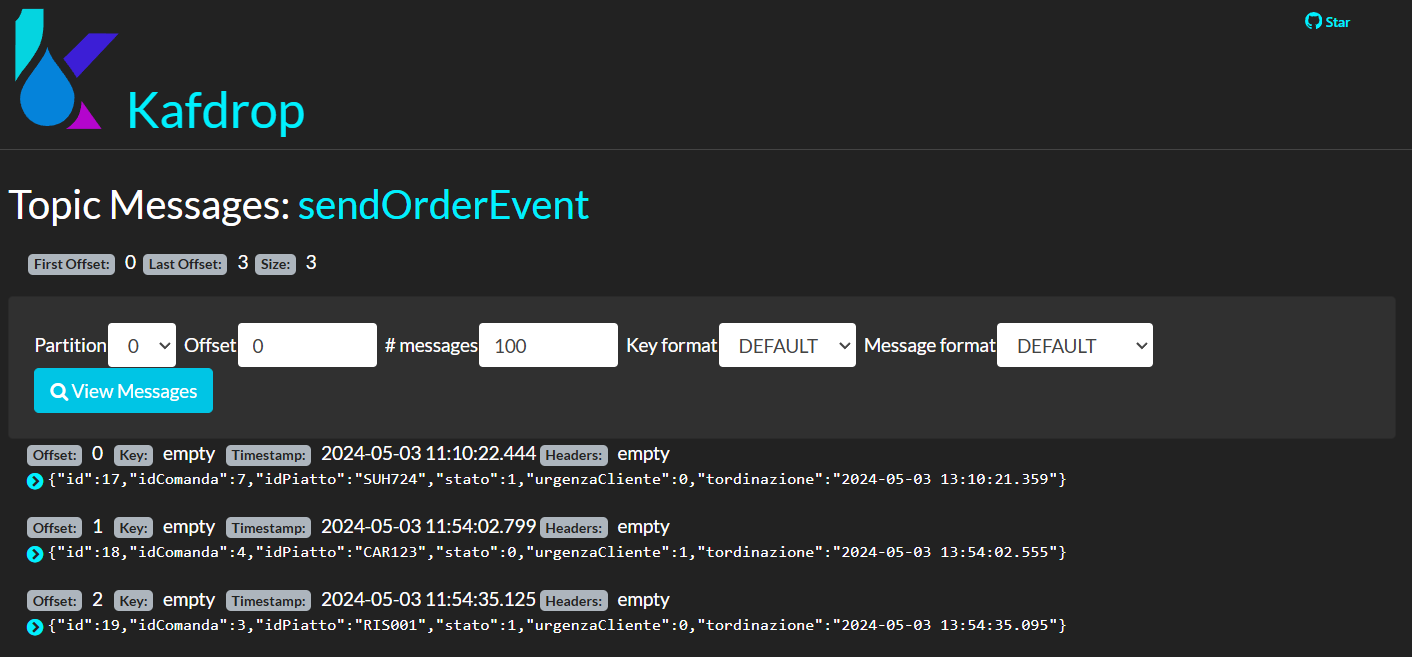
\includegraphics[width=1\linewidth]{iterazione1//images/kafdrop_esempio_funzionamento.png}
    \caption{Esempio funzionamento kafdrop}
    \label{fig:kafdrop_funzionamento}
\end{figure}
\paragraph{Step 5 - Testing}
In questo passo è stato creato il primo test di integrazione per il producer per verificare il corretto invio di un messaggio sul topic tramite il producer appena creato e la ricezione tramite un consumer simulato utilizzando un'istanza Embedded Kafka \cite{TestingKafka}.
Embedded Kafka è una libreria che fornisce istanze di Kafka e Confluent Schema Registry in memoria per eseguire i test, in modo da non dipendere da un server Kafka esterno.
Viene quindi integrata nel pom.xml (Codice \vref{lst:pom-xml2}) la seguente dipendenza:
\begin{lstlisting}[language=XML, caption={Aggiornamento dipendenze nel pom.xml per includere spring-kafka-test}, label=lst:pom-xml2]
<dependency>
    <groupId>org.springframework.kafka</groupId>
    <artifactId>spring-kafka-test</artifactId>
    <scope>test</scope>
</dependency>
\end{lstlisting}
E aggiornato l’application.properties specifico dei test  (Codice \vref{lst:application-properties1}):
\begin{lstlisting}[language=yaml, caption={Aggiornamento del file `application.properties` di test per il producer kafka}, label=lst:application-properties1]
spring.kafka.bootstrap-servers=localhost:9092
spring.kafka.consumer.auto-offset-reset= earliest
spring.kafka.producer.topic=test.topic.comanda
\end{lstlisting}
Fatto ciò si può procedere a scrivere la seguente classe di test (Codice \vref{lst:CucinaPubProducerTest}):
\begin{lstlisting}[style=myJava, 
    caption={Test di integrazione per il producer CucinaPubProducer}, label=lst:CucinaPubProducerTest, 
    emph={[2] kafkaTemplate , objectMapper, topic, payload, log, producer, embeddedKafka, logger, testAppender },
    emphstyle={[2]\color{codeDarkMagenta}},
    emph={[3] setup, testSendingMessage },
    emphstyle={[3]\color{codeCyan}}]
@EnableKafka
@SpringBootTest()
@DirtiesContext
@TestMethodOrder(MethodOrderer.OrderAnnotation.class)
@EmbeddedKafka(partitions = 1,
        controlledShutdown = false,
        brokerProperties = { "listeners=PLAINTEXT://localhost:9092", "port=9092" },
        topics = {"${spring.kafka.producer.topic}"})
class CucinaPubProducerTests {

    @Autowired
    private CucinaPubProducer producer;
    @Autowired
    private EmbeddedKafkaBroker embeddedKafka;
    @Autowired
    private ObjectMapper objectMapper;
    @Value("${spring.kafka.producer.topic}")
    private String topic;
    private Logger logger;
    private TestAppender testAppender;

    @BeforeEach
    public void setup() {
        logger = (Logger) LoggerFactory.getLogger(CucinaPubProducer.class);
        testAppender = new TestAppender();
        testAppender.start();
        logger.addAppender(testAppender);
    }

    @Test
    public void testSendingMessage() throws JsonProcessingException {

        OrdineDTO ordineDTO = TestDataUtil.createOrdineDtoA();

        producer.send(ordineDTO);
        String message = objectMapper.writeValueAsString(ordineDTO);

        // configurazione del consumer di Embedded Kafka
        Map<String, Object> consumerProps = KafkaTestUtils.consumerProps("testT", "false", embeddedKafka);
        DefaultKafkaConsumerFactory<Integer, String> cf = new DefaultKafkaConsumerFactory<>(consumerProps);
        Consumer<Integer, String> consumer = cf.createConsumer();
        embeddedKafka.consumeFromAnEmbeddedTopic(consumer, topic);
        ConsumerRecord<Integer, String> received = KafkaTestUtils.getSingleRecord(consumer, topic);

        // testo il corretto invio
        assertFalse(testAppender.events.isEmpty());
        assertEquals("Sent Message=[" + message + "] with offset=[0]", testAppender.events.get(0).getFormattedMessage());

        // testo la corretta ricezione
        assertThat(received.offset()).isEqualTo(0);
        assertThat(received.topic()).isEqualTo(topic);
        assertThat(received.partition()).isEqualTo(0);
        OrdineDTO ordineDTOReceived = objectMapper.readValue(received.value(),OrdineDTO.class);
        assertThat(ordineDTOReceived).isEqualTo(ordineDTO);

        logger.detachAppender(testAppender);
    }
}
\end{lstlisting}
Che testa il corretto invio di un oggetto creato tramite la classe di supporto testDataUtil e verifica inizialmente che il log della classe CucinaPubAdapter sia quello che ci si aspetta, mentre successivamente verifica che il consumer creato utilizzando un’istanza di EmbeddedKafka riceva l’oggetto inviato, viene di conseguenza testata anche la serializzazione.
\paragraph{Step 6 - Consumer}
Creato e testato il producer si è passati alla creazione di un consumer, inizialmente si è creato un consumer generico in ascolto sullo stesso topic del producer appena creato, verificato il funzionamento si è passati a creare i due producer richiesti in maniera speculare, di seguito verrà mostrato il producer in ascolto sul topic del microservizio di Gestione Cliente ossia SubClienteAdapter.
Come prima cosa si è aggiornato l’application.yml (Codice \vref{lst:application-yml2}) con la configurazione del consumer in questione:
\begin{lstlisting}[language=yaml, caption={Aggiornamento del file `application.yml` per il consumer Kafka}, label=lst:application-yml2]
kafka:
 consumer:
   gestioneCliente:
     topic: notifyOrderEvent
     group-id: gestioneCliente
\end{lstlisting}
Poi si è passati direttamente ad implementare la classe SubClienteAdapter (Codice: \vref{lst:subclienteadapter})  che implementa l'interfaccia NotifyOrderEvent (Codice: \vref{lst:notifyordereventIF})  
\begin{lstlisting}[style=myJava, 
    caption={Classe del consumer kafka SubClienteAdapter.java}, label=lst:subclienteadapter, 
    emph={[2] kafkaTemplate , objectMapper, topic, payload, log, producer, embeddedKafka, logger, testAppender, RECEIVED_TOPIC, RECEIVED_PARTITION, OFFSET, clientePort, lastMessageReceived, latch,  },
    emphstyle={[2]\color{codeDarkMagenta}},
    emph={[3] receive, resetLatch, getLatch, getLastMessageReceived },
    emphstyle={[3]\color{codeCyan}}]
@Component
@Log
public class SubClienteAdapter implements NotifyOrderEvent {

    private ObjectMapper objectMapper;
    private ClientePort clientePort;

    /**
     * variabile thread safe che serve per fini di test per verificare che il listener abbia ricevuto un messaggio
     */
    private CountDownLatch latch = new CountDownLatch(1);
    private final Logger logger = LoggerFactory.getLogger(SubCucinaAdapter.class);
    private NotificaOrdineDTO lastMessageReceived;

    @Autowired
    public SubClienteAdapter(final ClientePort clientePort, final ObjectMapper objectMapper) {
        this.clientePort = clientePort;
        this.objectMapper = objectMapper;
    }

    @Override
    public void receive(@Payload String message,
                        @Header(KafkaHeaders.RECEIVED_TOPIC) String topic,
                        @Header(KafkaHeaders.RECEIVED_PARTITION) Integer partition,
                        @Header(KafkaHeaders.OFFSET) Long offset) throws JsonProcessingException {
        logger.info("Received a message {}, from {} topic, " +
                "{} partition, and {} offset", message.toString(), topic, partition, offset);
        NotificaOrdineDTO notificaOrdineDTO = objectMapper.readValue(message, NotificaOrdineDTO.class);
        clientePort.notifyOrder(notificaOrdineDTO);
        lastMessageReceived = notificaOrdineDTO;
        latch.countDown();
    }

    /**
     * resetta il valore del latch
     */
    public void resetLatch() {
        latch = new CountDownLatch(1);
    }

    /**
     * restituisce il latch
     *
     * @return latch: variabile thread safe che serve per fini di test per verificare
     * che il listener abbia ricevuto un messaggio
     */
    public CountDownLatch getLatch() {
        return latch;
    }

    /**
     * Restituisce l'ultimo messaggio letto dal listener
     *
     * @return l'ultimo messaggio letto dal listener
     */
    @Override
    public NotificaOrdineDTO getLastMessageReceived() {
        return lastMessageReceived;
    }
}
\end{lstlisting}
Nella quale il metodo receive è annotato con @KafkaListener, questo permette di stare costantemente in ascolto sul topic specificato e svolgere il contenuto del metodo quando viene rilevato un messaggio, nello specifico si produce un log di corretta ricezione e si salva l’oggetto ricevuto. Inizialmente si è lavorato solamente tramite log con un messaggio “Hello world”, successivamente verificato il funzionamento si è passati a lavorare con oggetti e quindi viene effettuata la deserializzazione tramite \textit{objectMapper} e il salvataggio nel campo \textit{lastMessageReceived}. Per quanto riguarda il \textit{latch} è una variabile thread safe che serve a fini di test per verificare che il listener abbia ricevuto un messaggio utilizzando un comportamento sincrono, non viene coinvolta nel normale svolgimento dell’applicazione.
Si passa quindi alla fase di test per verificare che il consumer SubClienteAdapter stia in ascolto e riceva messaggi correttamente dal topic del message broker, inizialmente si configura l’application.properties (Codice \vref{lst:application-properties3}) di test con il topic di test del consumer:
\begin{lstlisting}[language=yaml, caption={Aggiornamento del file `application.properties` di test per il consumer Kafka}, label=lst:application-properties3]
spring.kafka.consumer.gestioneCliente.topic=test.topic.cliente
\end{lstlisting}
Poi in n modo analogo alla classe del producer viene creato il seguente test di integrazione (Codice \vref{lst:SubClienteAdapterTest}) sempre sfruttando Embedded Kafka:
\begin{lstlisting}[style=myJava, 
    caption={Test di integrazione per il consumer SubClienteAdapter}, label=lst:SubClienteAdapterTest,
    emph={[2] kafkaTemplate , objectMapper, topic, payload, log, producer, embeddedKafka, logger, testAppender,},
    emphstyle={[2]\color{codeDarkMagenta}},
    emph={[3] setup, testOutput1 },
    emphstyle={[3]\color{codeCyan}}]
@EnableKafka
@SpringBootTest
@DirtiesContext
@Log
@EmbeddedKafka(partitions = 1,
       controlledShutdown = false,
       brokerProperties = { "listeners=PLAINTEXT://localhost:9092", "port=9092" },
       topics = {"${spring.kafka.consumer.gestioneCliente.topic}"})
public class SubClienteAdapterTests {
   @Autowired
   private EmbeddedKafkaBroker embeddedKafka;
   @Autowired
   private SubClienteAdapter subClienteAdapter; // kafka consumer
   @Value("${spring.kafka.consumer.gestioneCliente.topic}")
   private String topic;
   private Logger logger;
   private TestAppender testAppender;

   @BeforeEach
   public void setup() {
       subClienteAdapter.resetLatch();
       logger = (Logger) LoggerFactory.getLogger(SubCucinaAdapter.class);
       testAppender = new TestAppender();
       testAppender.start();
       logger.addAppender(testAppender);
   }

   @Test
   public void testOutput1() throws Exception {
       NotificaOrdineDTO notificaOrdineDTO = TestDataUtil.createNotificaOrdineDTOA();
       String notifica = TestUtil.serialize(notificaOrdineDTO);

       CompletableFuture<SendResult<Integer, String>> future = TestUtil.sendMessageToTopic(topic,notifica,embeddedKafka);
       log.info("Sent Message=[" + notifica + "] with offset=[0]");

       boolean messageConsumed = subClienteAdapter.getLatch().await(10, TimeUnit.SECONDS);

       //testo il corretto invio
       future.whenComplete((result,ex)->{
           assertThat(ex).isNull(); 
           // verifica che non sia stata sollevata alcuna eccezione
       });

       // testo la corretta ricezione
       assertTrue(messageConsumed);
       assertFalse(testAppender.events.isEmpty());
       assertEquals("Received a message " + notifica + ", from " + topic + " topic, 0 partition, and 0 offset", testAppender.events.get(0).getFormattedMessage());

       NotificaOrdineDTO notificaOrdineDTOReceived = subClienteAdapter.getLastMessageReceived();
       assertEquals(notificaOrdineDTO, notificaOrdineDTOReceived);
       logger.detachAppender(testAppender);
   }
}
\end{lstlisting}
In questa classe di test si utilizza un’istanza di Embedded Kafka per simulare il producer, mentre come consumer si utilizza la classe sotto test SubClienteAdapter.
Si testa il corretto invio di un oggetto creato tramite la classe di supporto testDataUtil e si verifica che il producer invii effettivamente un messaggio sul topic, poi si verifica la ricezione verificando inizialmente che il log della classe SubClienteAdapter sia quello che ci si aspetta, mentre successivamente si verifica che riceva l’oggetto inviato, viene di conseguenza testata anche la deserializzazione.


\subsection{Creazione del Database}
TODO

\subsection{Adattatore JPA}
Lo sviluppo del componente adibito all'adattatore JPA è stato un processo che ha seguito vari step:
\paragraph{Step 1 - Overview:}
Come primo passo ci si è fatti una panoramica leggendo la documentazione ufficiale di Spring Data JPA \cite{spring-data-jpa} e si sono cercati alcuni progetti su Github di \href{https://github.com/spring-projects/spring-data-examples/}{esempio}.
\paragraph{Step 2 - Setup:}
Al passo numero due ci si è focalizzati sul setup dell’ambiente di lavoro, andando ad aggiornare il file "pom.xml" (Codice \vref{lst:pom-xml3}) con la seguente dipendenza per Spring Data JPA:
\begin{lstlisting}[language=XML, caption={Aggiornamento dipendenze nel pom.xml per includere spring-data-jpa}, label=lst:pom-xml3]
<dependency>
    <groupId>org.springframework.boot</groupId>
    <artifactId>spring-boot-starter-data-jpa</artifactId>
</dependency>
\end{lstlisting}
Successivamente nel file "application.yml" (Codice \vref{lst:application-yml3}) sono state aggiunte le seguenti istruzioni di configurazione:
\begin{lstlisting}[language=yaml, caption={Aggiornamento del file `application.yml` per Spring Data JPA}, label=lst:application-yml3]
spring:
  jpa:
    properties:
      hibernate:
        dialect: org.hibernate.dialect.MariaDBDialect
        temp:
          use_jdbc_metadata_defaults: false
    hibernate:
      ddl-auto: none #update
    show-sql: true
\end{lstlisting}
\paragraph{Step 3 - Entità:}
Nel passo successivo si è passati a creare la prima entità, le entità in Spring Boot JPA sono fondamentalmente POJOs (Plain Old Java Objects) che rappresentano dati che possono essere resi persistenti nel database. Ogni istanza di un’entità rappresenta una riga in una tabella del database. Si è definita quindi l'entità Ordine (Codice \vref{lst:OrdineEntity}) in questo modo:
\begin{lstlisting}[style=myJava, 
    caption={Classe entità OrdineEntity.java}, label=lst:OrdineEntity, 
    emph={[2] urgenzaCliente, id, idComanda, idPiatto, stato, tOrdinazione},
    emphstyle={[2]\color{codeDarkMagenta}}]
@Data
@AllArgsConstructor
@NoArgsConstructor
@Builder
@Entity
@Table(name = "Ordine", schema = "serveeasy", catalog = "")
public class OrdineEntity {
    /**
     * Identificatore dell'ordine
     */
    @GeneratedValue(strategy = GenerationType.IDENTITY)
    @Id
    @Column(name = "ID", nullable = false, insertable = false, updatable = false)
    private int id;

    /**
     * Identificatore della comanda di cui l'ordine fa parte
     */
    @Column(name = "ID_COMANDA", nullable = false, updatable = false)
    private int idComanda;

    /**
     * Identificatore del piatto ordinato dal cliente
     */
    @Basic
    @Column(name = "ID_piatto", nullable = false, length = 20)
    private String idPiatto;

    /**
     * Stato dell'ordine
     * 0: Ordine preso in carico
     * 1: Ordine in coda di preparazione
     * 2: Ordine in preparazione
     * 3: Ordine preparato
     */
    @Basic
    @Column(name = "stato", updatable = true)
    private Integer stato;

    /**
     * Istante temporale in cui viene effettuata l'ordinazione
     * pattern : "yyyy-MM-dd HH:mm:ss.SSS"
     */
    @Basic
    @CreationTimestamp
    @Column(name = "t_ordinazione", updatable = false)
    private Timestamp tOrdinazione;

    /**
     * Attributo urgenza del cliente
     * 0 : espresso non urgenza
     * 1 : espresso urgenza
     * 2 : default
     */
    @Basic
    @Column(name = "urgenza_cliente", updatable = true)
    private Integer urgenzaCliente;
}
\end{lstlisting}
Grazie alla alla notazione @Entity segnaliamo a JPA che questa classe è un’entità, con @Table  specifichiamo il nome della tabella nel database e con @Id definiamo la chiave primaria della entità.
\paragraph{Step 4 - Repository:}
Nello step 4 andiamo a definire una repository per la classe ordine, ossia un meccanismo per l’incapsulamento dello storage, recupero e comportamento di ricerca che emula una collezione di oggetti:
\begin{lstlisting}[style=myJava, 
    caption={Classe repository OrdineRepository.java}, label=lst:OrdineRepository, 
    emph={[3] findOrdineEntitiesByIdComanda },
    emphstyle={[3]\color{codeCyan}}]
@Repository
public interface OrdineRepository extends CrudRepository<OrdineEntity, Integer> {

    /**
     * Permette di ottenere una lista di Entita' Ordine con lo stesso id di comanda specificato
     *
     * @param idComanda codice identificativo della comanda
     * @return oggetto Iterable che punta a una lista contenente entita' ordine con lo stesso id di comanda specificato
     */
    Iterable<OrdineEntity> findOrdineEntitiesByIdComanda(int idComanda);
}
\end{lstlisting}
La classe OrdineRepository (Codice \vref{lst:OrdineRepository}) gestisce le operazioni CRUD (Create, Read, Update, Delete) per l’entità OrdineEntity, inoltre questa interfaccia definisce un metodo personalizzato:
\textit{findOrdineEntitiesByIdComanda(int idComanda)} che restituisce un Iterable di OrdineEntity che hanno lo stesso \textit{idComanda} specificato.
Spring Data JPA implementerà automaticamente questo metodo, non è quindi necessario fornire un’implementazione personalizzata a meno che non si desideri un comportamento specifico che non è coperto dalle convenzioni di denominazione di Spring Data JPA.
\paragraph{Step 5 - JPA Adapter:}
A questo punto siamo pronti per definire la classe adattatore di JPA JPADBAdapter.java (Codice \vref{lst:JPADBAdapter}) che implementa la DataPort (Codice \vref{lst:dataport}):
\begin{lstlisting}[style=myJava, 
    caption={Classe adattatore JPA JPADBAdapter.java}, label=lst:JPADBAdapter, 
    emph={[2] ordineRepository, log, logger},
    emphstyle={[2]\color{codeDarkMagenta}},
    emph={[3] JPADBAdapter, isOrderExist, saveOrder, getOrderById, updateOrder, findAllOrdersByIdComanda, deleteOrder },
    emphstyle={[3]\color{codeCyan}},]
@Repository
public class JPADBAdapter implements DataPort {

    private final OrdineRepository ordineRepository;

    @Autowired
    public JPADBAdapter(OrdineRepository ordineRepository) {
        this.ordineRepository = ordineRepository;
    }

    @Override
    public boolean isOrderExist(int id) {
        return ordineRepository.existsById(id);
    }

    @Override
    public OrdineEntity saveOrder(OrdineEntity ordineEntity) {
        return ordineRepository.save(ordineEntity);
    }

    @Override
    public Optional<OrdineEntity> getOrderById(int id) {
        return ordineRepository.findById(id);
    }

    @Override
    public OrdineEntity updateOrder(int id, OrdineEntity ordineEntity) {
        ordineEntity.setId(id);

        return ordineRepository.findById(ordineEntity.getId()).map(existingOrder -> {
            Optional.ofNullable(ordineEntity.getStato()).ifPresent(existingOrder::setStato);
            Optional.ofNullable(ordineEntity.getUrgenzaCliente()).ifPresent(existingOrder::setUrgenzaCliente);
            return ordineRepository.save(existingOrder);
        }).orElseThrow(() -> new RuntimeException("Order does not exist"));
    }

    @Override
    public List<OrdineEntity> findAllOrdersByIdComanda(int idComanda) {
        return StreamSupport.stream(ordineRepository.findOrdineEntitiesByIdComanda(idComanda).spliterator(), false).collect(Collectors.toList());
    }

    @Override
    public void deleteOrder(int id) {
        ordineRepository.deleteById(id);
    }
}
\end{lstlisting}
Questa classe funge da adattatore tra il database e l'applicazione, fornendo un’implementazione dei metodi definiti nell’interfaccia DataPort, consentendo operazioni di accesso ai dati per l'entità ordine. È possibile notare come viene utilizzato l'oggetto istanza della classe OrdineRepository definita poc'anzi (Codice \vref{lst:OrdineRepository}) per eseguire operazioni di persistenza dei dati relativi agli ordini senza aver fornito un'implementazione, ma lasciando questo compito a Spring Data JPA.
\paragraph{Step 6 - Testing:}
In questo passo si sono svolti i test sulla DataPort per verificare il corretto funzionamento dell'adattatore JPA correlato. Per eseguire i test si è utilizzato un database H2\cite{H2DB} in memoria poichè offre velocità, isolamento, semplicità di configurazione e indipendenza dall'infrastruttura esterna, rendendo i test più efficienti e affidabili. Quindi come prima cosa si integra la dipendenza di H2 nel file "pom.xml" (Codice \vref{lst:pom-xml4}) in questo modo:
\begin{lstlisting}[language=xml, caption={Aggiornamento del file pom.xml per la dipendenza di H2}, label=lst:pom-xml4]
<dependency>
    <groupId>com.h2database</groupId>
    <artifactId>h2</artifactId>
    <scope>runtime</scope>
</dependency>
\end{lstlisting}
Poi si aggiorna il file application.properties (Codice \vref{lst:application-properties-test3}) specifico dei test come segue:
\begin{lstlisting}[language=yaml, caption={Aggiornamento del file application.properties per i test con H2}, label=lst:application-properties-test3]
spring.jpa.properties.hibernate.dialect=org.hibernate.dialect.MariaDBDialect
spring.jpa.hibernate.ddl-auto=create-drop
spring.jpa.show-sql=true
# H2 Database in memory to simulate MariaDB
spring.datasource.url=jdbc:h2:mem:testdb;MODE=MariaDB;DATABASE_TO_LOWER=TRUE
spring.datasource.username=user
spring.datasource.password=user
spring.datasource.driver-class-name=org.h2.Driver
\end{lstlisting}
A questo punto si può passare a creare il test di integrazione della DataPort (Codice \vref{lst:DataPortTest}):
\begin{lstlisting}[style=myJava, 
    caption={Classe adattatore JPA JPADBAdapter.java}, label=lst:DataPortTest, 
    emph={[2] dataPort, log, logger, AFTER_EACH_TEST_METHOD},
    emphstyle={[2]\color{codeDarkMagenta}},
    emph={[3] testSaveOrderAndFindOrderById, testMultipleSaveOrderAndFindByIdComanda, testOrderPartialUpdate, testDeleteOrder },
    emphstyle={[3]\color{codeCyan}},]
@SpringBootTest
@ExtendWith(SpringExtension.class)
@DirtiesContext(classMode = DirtiesContext.ClassMode.AFTER_EACH_TEST_METHOD)
public class DataPortTests {

    private DataPort dataPort;

    @Autowired
    public DataPortTests(DataPort dataPort) {
        this.dataPort = dataPort;
    }

    @Test
    public void testSaveOrderAndFindOrderById() {
        OrdineEntity ordineEntity = TestDataUtil.createOrdineEntityA();
        OrdineEntity savedOrdineEntity = dataPort.saveOrder(ordineEntity);
        Optional<OrdineEntity> result = dataPort.getOrderById(savedOrdineEntity.getId());
        assertThat(result).isPresent();
        assertThat(result.get()).isEqualTo(savedOrdineEntity);
        assertThat(result.get().getId()).isEqualTo(1);
        assertThat(result.get().getIdComanda()).isEqualTo(ordineEntity.getIdComanda());
        assertThat(result.get().getStato()).isEqualTo(ordineEntity.getStato());
        assertThat(result.get().getIdPiatto()).isEqualTo(ordineEntity.getIdPiatto());
        assertThat(result.get().getTOrdinazione()).isEqualTo(ordineEntity.getTOrdinazione());
    }

    @Test
    public void testMultipleSaveOrderAndFindByIdComanda(){
        OrdineEntity ordineEntityA = TestDataUtil.createOrdineEntityA();
        OrdineEntity savedOrdineEntityA = dataPort.saveOrder(ordineEntityA);
        OrdineEntity ordineEntityB = TestDataUtil.createOrdineEntityB();
        OrdineEntity savedOrdineEntityB = dataPort.saveOrder(ordineEntityB);
        OrdineEntity ordineEntityC = TestDataUtil.createOrdineEntityC();
        OrdineEntity savedOrdineEntityC = dataPort.saveOrder(ordineEntityC);

        Iterable<OrdineEntity> result = dataPort.findAllOrdersByIdComanda(ordineEntityA.getIdComanda());
        assertThat(result).hasSize(2).containsExactly(savedOrdineEntityA, savedOrdineEntityB);
    }

    @Test
    public void testOrderPartialUpdate() {
        OrdineEntity ordineEntity = TestDataUtil.createOrdineEntityA();
        OrdineEntity savedOrdineEntity = dataPort.saveOrder(ordineEntity);
        savedOrdineEntity.setStato(0);
        savedOrdineEntity.setUrgenzaCliente(1);
        dataPort.saveOrder(savedOrdineEntity);
        Optional<OrdineEntity> result = dataPort.getOrderById(savedOrdineEntity.getId());
        assertThat(result).isPresent();
        assertThat(result.get()).isEqualTo(savedOrdineEntity);
    }

    @Test
    public void testDeleteOrder() {
        OrdineEntity ordineEntityA = TestDataUtil.createOrdineEntityA();
        OrdineEntity savedOrdineEntityA = dataPort.saveOrder(ordineEntityA);
        dataPort.deleteOrder(savedOrdineEntityA.getId());
        Optional<OrdineEntity> result = dataPort.getOrderById(savedOrdineEntityA.getId());
        assertThat(result).isEmpty();
    }
}
\end{lstlisting}
In questa classe di test vengono testate tutte e 4 le operazioni CRUD, ossia Create (Creazione), Read (Lettura), Update (Aggiornamento) e Delete (Eliminazione) per mezzo della DataPort e quindi della sua implementazione JPADBAdapter (\vref{lst:JPADBAdapter}) verso il database, le entità vengono create tramite una classe di supporto TestDataUtil e la DataPort viene iniettata tramite il costruttore grazie all'annotazione @Autowired.

% TODO non so se qui integrare la UI per il DB o al passo precedente

\subsection{Continuous Integration}
Una volta creati tutti gli adattatori principali l'attenzione si è spostata ad introdurre tecniche di Continuous Integration (CI), la CI è una pratica di sviluppo software che prevede che i membri di un team integrino frequentemente il loro lavoro in un repository condiviso, al fine di rilevare e risolvere rapidamente eventuali problemi o conflitti nel codice.
\paragraph{Step 1 - Overview:}
Come primo passo ci si è fatti una panoramica leggendo la documentazione ufficiale di GitHub Actions \cite{ContinuousIntegrationGithubActions}.
\paragraph{Step 2 - Setup:}
Al passo numero due ci si è focalizzati sul setup dell’ambiente di lavoro, andando a creare la cartella \href{https://github.com/giorgio-hash/GestioneComanda/tree/main/.github/workflows}{".github/workflows"} nella repository principale di Gestione Comanda e creando il file "maven.yml" (Codice \vref{lst:maven-yml}) come segue:
\begin{lstlisting}[language=yaml, caption={Creazione del file maven.yml}, label=lst:maven-yml]
name: Java CI with Maven

on:
  push:
    branches: [ "*" ]
  pull_request:
    branches: [ "main" ]

jobs:
  build:
    runs-on: ubuntu-latest
    
    if: github.ref != 'refs/heads/main'
    steps:
    - uses: actions/checkout@v4
    - name: Set up JDK 17
      uses: actions/setup-java@v4
      with:
        java-version: '17'
        distribution: 'temurin'
        cache: maven
    - name: Run the Maven verify phase
      run: mvn --batch-mode clean verify
\end{lstlisting}
Questo flusso di lavoro configura l'ambiente di esecuzione, scarica il codice sorgente del progetto, imposta il JDK 17 ed infine esegue i test del progetto utilizzando Maven. È un'applicazione di CI che garantisce che il codice sia testato automaticamente ogni volta che vengono apportate modifiche su ogni branch e ogni volta che si effettua una pull-request verso il main.
\paragraph{Step 3 - Testing:}
Per testare il funzionamento basta fare il push di un commit verso la cartella remota di GitHub o eseguire una pull-request verso il main, prendiamo in considerazione questo esempio in cui si esegue la seconda delle due opzioni appena citate:
\begin{figure}[H]
    \centering
    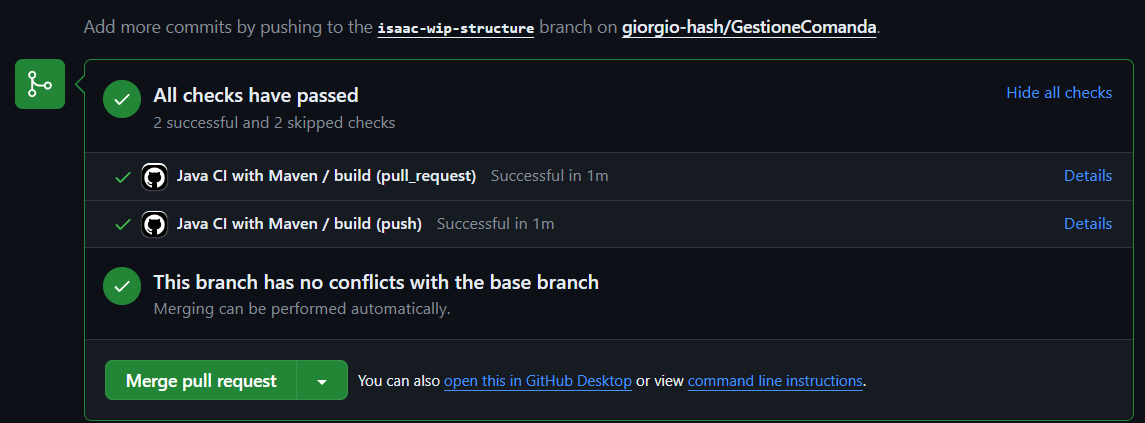
\includegraphics[width=1\linewidth]{iterazione1//images/github_actions_merge.png}
    \caption{CI merge a pull-request}
    \label{fig:cigithubmerge}
\end{figure}
Dalla Figura \vref{fig:cigithubmerge} è possibile notare come all'interno della pull-request sia presente un campo dedicato ai controlli che GitHub Actions ha effettuato e siccome tutti i controlli hanno avuto esito positivo, è possibile procedere al merge della richiesta.
\begin{figure}[H]
    \centering
    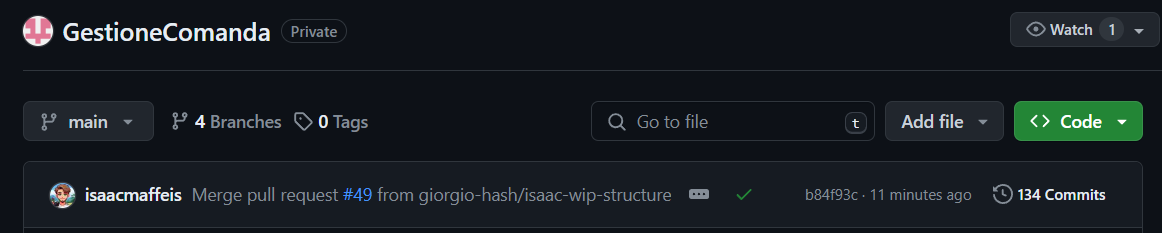
\includegraphics[width=1\linewidth]{iterazione1//images/github_actions_main}
    \caption{CI main check}
    \label{fig:cigithubmain}
\end{figure}
Una volta completato il merge con successo è possibile notare una spunta verde nella repository principale del progetto (Figura \vref{fig:cigithubmain}) che ci informa che allo stato corrente il codice sul main ha passato tutti i test proposti.

\subsection{DTO}
Gli oggetti di trasferimento dati (Data Transfer Object) sono un design pattern utilizzato per trasferire dati tra sottosistemi di un’applicazione software, servono a semplificare e a rendere più efficiente la comunicazione tra i vari livelli di un'applicazione, nel nostro caso tra Interface, Domain e Infrastructure.
\paragraph{Step 1 - Overview:}
Come primo passo ci si è fatti una panoramica leggendo la documentazione ufficiale di Model Mapper \cite{ModelMapperGettingStarted}, ossia la libreria di mapping che useremo per convertire le entità in DTO e viceversa.
\paragraph{Step 2 - Setup:}
Al passo numero due ci si è focalizzati sul setup dell’ambiente di lavoro, andando ad aggiornare inizialmente il file "pom.xml" (Codice \vref{lst:pom-xml5}) con la seguente dipendenza per Model Mapper:
\begin{lstlisting}[language=XML, caption={Aggiornamento dipendenze nel pom.xml per includere model-mapper}, label=lst:pom-xml5]
<dependency>
    <groupId>org.modelmapper</groupId>
    <artifactId>modelmapper</artifactId>
    <version>3.0.0</version>
</dependency>
\end{lstlisting}
E successivamente è stato creato il bean di configurazione nella classe "MapperConfig.java" (Codice \vref{lst:MapperConfig}):
\begin{lstlisting}[style=myJava, 
    caption={Classe di configurazione MapperConfig.java}, label=lst:MapperConfig, 
    emph={[2] LOOSE},
    emphstyle={[2]\color{codeDarkMagenta}},]
@Configuration
public class MapperConfig {

    @Bean
    ModelMapper modelMapper(){
        ModelMapper modelMapper = new ModelMapper();
        modelMapper.getConfiguration().setMatchingStrategy(MatchingStrategies.LOOSE);
        return modelMapper;
    }
}
\end{lstlisting}
La strategia di corrispondenza LOOSE in ModelMapper ignora le differenze di maiuscole/minuscole e gli underscore nei nomi dei campi, considera i campi come corrispondenti anche se i nomi dei campi nell’oggetto sorgente e nell’oggetto destinazione non sono esattamente gli stessi, ma contengono le stesse parole.
\paragraph{Step 3 - DTO:}
Al terzo passo è stata creata la classe DTO per l'entità Ordine che abbiamo definito in precedenza (Codice \vref{lst:OrdineEntity}), semplicemente creando una nuova classe Java (Codice \vref{lst:orderdto}) con gli stessi campi della classe entità, ma senza la logica di business o le annotazioni specifiche dell'entità:
\begin{lstlisting}[style=myJava, 
    caption={Classe DTO per l'entità ordine OrderDTO.java}, label=lst:orderdto, 
    emph={[2] urgenzaCliente, id, idComanda, idPiatto, stato, tOrdinazione },
    emphstyle={[2]\color{codeDarkMagenta}},]
@Data
@AllArgsConstructor
@NoArgsConstructor
@Builder
public class OrdineDTO {

    /**
     * Identificatore dell'ordine
     */
    private int id;

    /**
     * Identificatore della comanda di cui l'ordine fa parte
     */
    private int idComanda;

    /**
     * Identificatore del piatto ordinato dal cliente
     */
    private String idPiatto;

    /**
     * Stato dell'ordine
     * 0: Ordine preso in carico
     * 1: Ordine in coda di preparazione
     * 2: Ordine in preparazione
     * 3: Ordine preparato
     */
    private Integer stato;

    /**
     * Istante temporale in cui viene effettuata l'ordinazione
     * pattern : "yyyy-MM-dd HH:mm:ss.SSS"
     */
    private Timestamp tOrdinazione;

    /**
     * Attributo urgenza del cliente
     * 0 : espresso non urgenza
     * 1 : espresso urgenza
     * 2 : default
     */
    private Integer urgenzaCliente;

}
\end{lstlisting}
\paragraph{Step 4 - Mapper:}
Le classi mapper sono utilizzate per convertire oggetti tra classi entità e DTO (e viceversa), viene inizialmente creata la seguente interfaccia (Codice \vref{lst:mapper}):
\begin{lstlisting}[style=myJava, 
    caption={Interfaccia Mapper.java}, label=lst:mapper, 
    emph={[3] A, B },
    emphstyle={[3]\color{codeCyan}},]
public interface Mapper<A,B> {

    /**
     * Mappa l'oggetto A (Entita') nell'oggetto B (DTO)
     *
     * @param a A Entita'
     * @return B DTO
     */
    B mapTo(A a);

    /**
     * Mappa l'oggetto B (DTO) nell'oggetto A (Entita')
     *
     * @param b B DTO
     * @return A Entita'
     */
    A mapFrom(B b);
\end{lstlisting}
Nella quale con \textit{mapTo} possiamo passare da un'entità ad un DTO, mentre con \textit{mapFrom} possiamo convertire un DTO in un'entità. Viene di conseguenza creata la classe implementazione di questa interfaccia (Codice \vref{lst:OrdineMapper}): 
\begin{lstlisting}[style=myJava, 
    caption={Classe OrdineMapper.java implementazione di ModelMapper.java}, label=lst:OrdineMapper, 
    emph={[2] modelMapper},
    emphstyle={[2]\color{codeDarkMagenta}},
    emph={[3] mapTo, mapFrom },
    emphstyle={[3]\color{codeCyan}},]
@Component
public class OrdineMapper implements Mapper<OrdineEntity, OrdineDTO> {

    private ModelMapper modelMapper;

    public OrdineMapper(ModelMapper modelMapper) {
        this.modelMapper = modelMapper;
    }

    @Override
    public OrdineDTO mapTo(OrdineEntity ordineEntity) {
        return modelMapper.map(ordineEntity,OrdineDTO.class);
    }

    @Override
    public OrdineEntity mapFrom(OrdineDTO ordineDTO) {
        return modelMapper.map(ordineDTO, OrdineEntity.class);
    }
}
\end{lstlisting}
Si può facilmente notare come l'utilizzo di ModelMapper abbia semplificato notevolmente il processo di mapping, infatti ci basta richiamare il metodo \textit{map} offerto dall'istanza modelMapper per svolgere la conversione tra due oggetti.
\paragraph{Step 5 - Testing:}
In questo passo sono stati svolti i test di integrazione (Codice \vref{lst:OrdineMapperTests}) per verificare che la conversione tra entità e DTO sia stata implementata in modo corretto.
\begin{lstlisting}[style=myJava, 
    caption={Test di integrazione OrdineMapperTests.java}, label=lst:OrdineMapperTests, 
    emph={[2] ordineMapper},
    emphstyle={[2]\color{codeDarkMagenta}},
    emph={[3] testMapTo, testMapFrom },
    emphstyle={[3]\color{codeCyan}},]
@SpringBootTest
public class OrdineMapperTests {

    @Autowired
    private OrdineMapper ordineMapper;

    @Test
    public void testMapTo(){
        OrdineEntity ordineEntity = TestDataUtil.createOrdineEntityA();
        OrdineDTO ordineDTO = ordineMapper.mapTo(ordineEntity);
        assertThat(ordineDTO.getId()).isEqualTo(ordineEntity.getId());
        assertThat(ordineDTO.getIdComanda()).isEqualTo(ordineEntity.getIdComanda());
        assertThat(ordineDTO.getStato()).isEqualTo(ordineEntity.getStato());
        assertThat(ordineDTO.getIdPiatto()).isEqualTo(ordineEntity.getIdPiatto());
        assertThat(ordineDTO.getUrgenzaCliente()).isEqualTo(ordineEntity.getUrgenzaCliente());
        assertThat(ordineDTO.getTOrdinazione()).isEqualTo(ordineEntity.getTOrdinazione());
    }

    @Test
    public void testMapFrom(){
        OrdineDTO ordineDTO = TestDataUtil.createOrdineDtoB();
        OrdineEntity ordineEntity = ordineMapper.mapFrom(ordineDTO);
        assertThat(ordineEntity.getId()).isEqualTo(ordineDTO.getId());
        assertThat(ordineEntity.getIdComanda()).isEqualTo(ordineDTO.getIdComanda());
        assertThat(ordineEntity.getStato()).isEqualTo(ordineDTO.getStato());
        assertThat(ordineEntity.getIdPiatto()).isEqualTo(ordineDTO.getIdPiatto());
        assertThat(ordineEntity.getUrgenzaCliente()).isEqualTo(ordineDTO.getUrgenzaCliente());
        assertThat(ordineEntity.getTOrdinazione()).isEqualTo(ordineDTO.getTOrdinazione());
    }
}
\end{lstlisting}
Il metodo \textit{testMapTo()} verifica che l'operazione di mappatura da OrdineEntity a OrdineDTO produca risultati attesi, mentre il metodo \textit{testMapFrom()} verifica che l'operazione inversa di mappatura da OrdineDTO a OrdineEntity produca risultati attesi, in entrambi i casi si considerano dei test di equivalenza su tutti i campi degli oggetti.
\subsection{Interfaccia di Test}
\label{subsec:interfaccia-test}
\paragraph{Step 1 - Overview:}
Come primo passo ci si è fatti una panoramica leggendo la documentazione ufficiale di Spring per costruire un controller REST \cite{spring-rest}.
\paragraph{Step 2 - Setup:}
Al passo numero due ci si è focalizzati sul setup dell’ambiente di lavoro, siccome il microservizio GestioneComanda è sprovvisto di un componente HTTP Controller nella sua Interfaccia (che contiene solo EventController), viene creato un controller di TEST per interagire direttamente con i componenti del servizio per i soli fini di test, per questo motivo viene aggiornato il diagramma UML di Interface di GestioneComanda come segue (Figura \vref{fig:component_comanda_w_test-GestioneComanda__Interface}):
\subsubsection*{zoom-in interface di gestione comanda}
\begin{figure}[H]
	\centering
	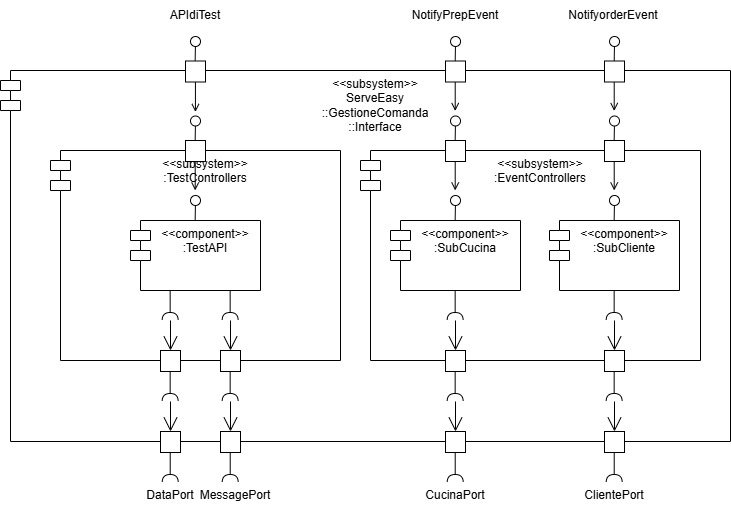
\includegraphics[scale=0.5]{iterazione1/images/component_comanda_w_test-GestioneComanda__Interface.jpg}
	\caption{Component diagram - Gestione Comanda - Interface con Test
    \label{fig:component_comanda_w_test-GestioneComanda__Interface}}
\end{figure}
\begin{itemize}
    \item EventControllers: SubCucina e SubCliente, permettono la ricezione di messaggi tramite message broker dagli altri microservizi.
    \item TestControllers: TestAPI per poter testare le API di Test utilizzando direttamente la DataPort e la MessagePort
\end{itemize}
Risulta importante specificare come il componente \textit{TestAPI} utilizzi direttamente la \textit{DataPort} e la \textit{MessagePort} invece che passare per le interfacce \textit{CucinaPort} e \textit{ClientePort} ovverte dal \textit{Domain}, questo viene fatto per non sconvolgere l'intera struttura dell'applicazione per i soli fini di test, infatti questo componente non verrà utilizzato in produzione.

Successivamente viene aggiornato il file "pom.xml"(Codice \vref{lst:pom-xml6}) con le seguenti dipendenze:
\begin{lstlisting}[language=XML, caption={Aggiornamento dipendenze nel pom.xml per includere spring-web}, label=lst:pom-xml6]
<!-- Spring web -->
<dependency>
    <groupId>org.springframework.boot</groupId>
    <artifactId>spring-boot-starter-web</artifactId>
</dependency>

<!-- Jackson -->
<dependency>
    <groupId>com.fasterxml.jackson.core</groupId>
    <artifactId>jackson-databind</artifactId>
</dependency>

<dependency>
    <groupId>com.fasterxml.jackson.datatype</groupId>
    <artifactId>jackson-datatype-jsr310</artifactId>
</dependency>
\end{lstlisting}
La prima (Spring web) è utilizzata per configurare un'applicazione Spring Boot che presenta un controller REST, include infatti tutte le dipendenze necessarie per avviare un'applicazione web, inclusi Tomcat, Spring MVC e altre dipendenze di supporto.
Mentre le seconde (Jackson) sono dipendenze Jackson utilizzate per la serializzazione e deserializzazione degli oggetti Java in formato JSON e viceversa fondamentali quando si sviluppano servizi RESTful con Spring Boot.
\paragraph{Step 3 - API:}
In questo passo vengono definite le API di Test che dovrà esporre il TestController, viene quindi creata l'interfaccia (Codice \vref{lst:testapiIF}) annotandola con \textit{@RequestMapping("/test")}, il che significa che tutti gli endpoint definiti all'interno di questa interfaccia sono raggiungibili tramite l'URI base "/test":
\begin{lstlisting}[style=myJava, 
    caption={Interfaccia TestAPI.java}, label=lst:testapiIF, 
    emph={[2] },
    emphstyle={[2]\color{codeDarkMagenta}},
    emph={[3] addOrdine, getOrdine, getAllOrdersByIdComanda, partialUpdateOrdine, deleteOrder, sendOrderEvent, getMessageFromTopicSendOrderEvent, sendNotifyOrderEvent, getMessageFromTopicNotifyOrderEvent, sendNotifyPrepEvent, getMessageFromTopicNotifyPrepEvent },
    emphstyle={[3]\color{codeCyan}},]
@RequestMapping("/test")
public interface TestAPI {

    /**
     * Salva nel database l'oggetto ordine dato un ordineDTO
     *
     * @param ordineDTO DTO dell'entita' ordine da salvare
     * @return entita' risposta che contiene l'oggetto creato e una risposta HTTP associata
     */
    @PostMapping(path="/order")
    ResponseEntity<OrdineDTO> addOrdine(@RequestBody OrdineDTO ordineDTO);

    /**
     * Restituisci l'ordine corrispondente all'id dato in input
     *
     * @param id id dell'ordine riqchiesto
     * @return entita' risposta che contiene l'oggetto richiesto e una risposta HTTP associata
     */
    @GetMapping(path="order/{id}")
    ResponseEntity<OrdineDTO> getOrdine(@PathVariable int id);

    /**
     * Restituisce una lista con tutti gli ordini relativi a una data comanda
     *
     * @param idComanda id della comanda di riferimento
     * @return entita' risposta che contiene la lista richiesta e una risposta HTTP associata
     */
    @GetMapping(path = "orders/{idComanda}")
    ResponseEntity<List<OrdineDTO>> getAllOrdersByIdComanda(@PathVariable int idComanda);

    /**
     * Aggiornamento parziale dell'entita' ordine, e' possibile fornire solamente gli oggetti da aggiornare
     *
     * @param id id dell'ordine da aggiornare
     * @param ordineDTO oggetto DTO con le modifiche da effettuare
     * @return entita' risposta che contiene l'oggetto aggiornato e una risposta HTTP associata
     */
    @PatchMapping(path="order/{id}")
    ResponseEntity<OrdineDTO> partialUpdateOrdine(@PathVariable int id, @RequestBody OrdineDTO ordineDTO);

    /**
     * Cancella l'ordine con il dato ID dal databse
     *
     * @param id id dell'ordine da eliminare
     * @return entita' risposta che contiene la risposta HTTP associata
     */
    @DeleteMapping(path = "/order/{id}")
    ResponseEntity deleteOrder(@PathVariable("id") int id);

    /**
     * Espone una API di POST con la quale e' possibile iniettare all'interno del broker oggetti al fine di test
     * Si testa il topic sendOrderEvent da gestione comanda verso gestione cucina
     *
     * @param ordineDTO contenuto dell'oggetto da iniettare
     * @return entita' risposta che contiene l'oggetto creato e una risposta HTTP associata
     * @throws JsonProcessingException eccezione sollevata dalla serializzazione
     */
    @PostMapping(path = "/sendorderevent")
    ResponseEntity<OrdineDTO> sendOrderEvent(@RequestBody OrdineDTO ordineDTO) throws JsonProcessingException;

    /**
     * Espone una API di GET con la quale e' possibile ottenere l'ultimo messaggio letto sul topic SendOrderEvent
     * Si testa il topic notifyPrepEvent da gestione cucina verso gestione comanda
     * @return entita' risposta che contiene l'oggetto richiesto e una risposta HTTP associata
     */
    @GetMapping(path = "/sendorderevent")
    ResponseEntity<String> getMessageFromTopicSendOrderEvent();

    /**
     * Espone una API di POST con la quale e' possibile iniettare all'interno del broker oggetti al fine di test
     * Si testa il topic notifyOrderEvent da gestione cliente verso gestione comanda
     * @param notificaOrdineDTO contenuto dell'oggetto da iniettare
     * @return entita' risposta che contiene l'oggetto creato e una risposta HTTP associata
     * @throws JsonProcessingException eccezione sollevata dalla serializzazione
     */
    @PostMapping(path = "/notifyorderevent")
    ResponseEntity<NotificaOrdineDTO> sendNotifyOrderEvent(@RequestBody NotificaOrdineDTO notificaOrdineDTO) throws JsonProcessingException;

    /**
     * Espone una API di GET con la quale e' possibile ottenere l'ultimo messaggio letto sul topic NotifyOrderEvent
     * Si testa il topic notifyPrepEvent da gestione cucina verso gestione comanda
     * @return entita' risposta che contiene l'oggetto richiesto e una risposta HTTP associata
     */
    @GetMapping(path = "/notifyorderevent")
    ResponseEntity<NotificaOrdineDTO> getMessageFromTopicNotifyOrderEvent();

    /**
     * Espone una API di POST con la quale e' possibile iniettare all'interno del broker oggetti al fine di test
     * Si testa il topic notifyPrepEvent da gestione cucina verso gestione comanda
     * @param notificaPrepOrdineDTO contenuto dell'oggetto da iniettare
     * @return entita' risposta che contiene l'oggetto creato e una risposta HTTP associata
     * @throws JsonProcessingException eccezione sollevata dalla serializzazione
     */
    @PostMapping(path = "/notifyprepevent")
    ResponseEntity<NotificaPrepOrdineDTO> sendNotifyPrepEvent(@RequestBody NotificaPrepOrdineDTO notificaPrepOrdineDTO) throws JsonProcessingException;

    /**
     * Espone una API di GET con la quale e' possibile ottenere l'ultimo messaggio letto sul topic NotifyPrepEvent
     * Si testa il topic notifyPrepEvent da gestione cucina verso gestione comanda
     * @return entita' risposta che contiene l'oggetto richiesto e una risposta HTTP associata
     */
    @GetMapping(path = "/notifyprepevent")
    ResponseEntity<NotificaPrepOrdineDTO> getMessageFromTopicNotifyPrepEvent();
}
\end{lstlisting}
In questo modo definiamo una serie di endpoint per API REST. Ogni metodo dell'interfaccia rappresenta un endpoint dell'API e specifica il tipo di richiesta HTTP supportata, il percorso dell'endpoint e gli eventuali parametri richiesti.
\paragraph{Step 4 - RestController:}
A questo punto possiamo costruire l'implementazione dell'interfaccia TestAPI appena definita (Codice \vref{lst:testapiIF}) andando a creare un controller REST di test (Codice \vref{lst:restcontrollertest}):
\begin{lstlisting}[style=myJava, 
    caption={Classe REST Controller di test TestController.java}, label=lst:restcontrollertest, 
    emph={[2] ordineMapper, testService, dataPort, topic_notifyOrderEvent, topic_notifyPrepEvent},
    emphstyle={[2]\color{codeDarkMagenta}},
    emph={[3] addOrdine, getOrdine, getAllOrdersByIdComanda, partialUpdateOrdine, deleteOrder, sendOrderEvent, getMessageFromTopicSendOrderEvent, sendNotifyOrderEvent, getMessageFromTopicNotifyOrderEvent, sendNotifyPrepEvent, getMessageFromTopicNotifyPrepEvent },
    emphstyle={[3]\color{codeCyan}},]
@RestController
public class TestController implements TestAPI {
    private TestService testService;
    private Mapper<OrdineEntity, OrdineDTO> ordineMapper;
    private DataPort dataPort;
    @Value("${spring.kafka.consumer.gestioneCliente.topic}")
    private String topic_notifyOrderEvent;
    @Value("${spring.kafka.consumer.gestioneCucina.topic}")
    private String topic_notifyPrepEvent;
    
    @Autowired
    public TestController(TestService testService, Mapper<OrdineEntity, OrdineDTO> ordineMapper, DataPort dataPort) {
        this.testService = testService;
        this.ordineMapper = ordineMapper;
        this.dataPort = dataPort;
    }

    @Override
    public ResponseEntity<OrdineDTO> addOrdine(OrdineDTO ordineDTO) {
        OrdineEntity ordineEntity = ordineMapper.mapFrom(ordineDTO);
        OrdineEntity savedOrdineEntity = dataPort.saveOrder(ordineEntity);
        OrdineDTO savedOrdineDTO = ordineMapper.mapTo(savedOrdineEntity);
        return new ResponseEntity<>(savedOrdineDTO, HttpStatus.CREATED);
    }

    @Override
    public ResponseEntity<OrdineDTO> getOrdine(int id) {
        Optional<OrdineEntity> ordineEntity = dataPort.getOrderById(id);
        if(ordineEntity.isPresent()){
            OrdineDTO ordineDTO = ordineMapper.mapTo(ordineEntity.get());
            return new ResponseEntity<>(ordineDTO, HttpStatus.OK);
        }
        return new ResponseEntity<>(HttpStatus.NOT_FOUND);
    }

    @Override
    public ResponseEntity<OrdineDTO> partialUpdateOrdine(@PathVariable int id, @RequestBody OrdineDTO ordineDTO) {
        if(!dataPort.isOrderExist(id))
            return new ResponseEntity<>(HttpStatus.NOT_FOUND);

        OrdineEntity ordineEntity = ordineMapper.mapFrom(ordineDTO);
        OrdineEntity updatedEntity = dataPort.updateOrder(id, ordineEntity);

        return new ResponseEntity<>(ordineMapper.mapTo(updatedEntity),HttpStatus.OK);
    }

    @Override
    public ResponseEntity<List<OrdineDTO>> getAllOrdersByIdComanda(int idComanda) {
        List<OrdineEntity> ordini = dataPort.findAllOrdersByIdComanda(idComanda);
        if(!ordini.isEmpty())
            return new ResponseEntity<>(ordini.stream()
                    .map(ordineMapper::mapTo)
                    .collect(Collectors.toList()),HttpStatus.OK);
        else
            return new ResponseEntity<>(HttpStatus.NOT_FOUND);
    }

    @Override
    public ResponseEntity deleteOrder(@PathVariable("id") int id) {
        dataPort.deleteOrder(id);
        return new ResponseEntity(HttpStatus.NO_CONTENT);
    }

    @Override
    public ResponseEntity<OrdineDTO> sendOrderEvent(@RequestBody OrdineDTO ordineDTO) throws JsonProcessingException {
        OrdineEntity ordineEntity = ordineMapper.mapFrom(ordineDTO);
        OrdineEntity savedOrdineEntity = dataPort.saveOrder(ordineEntity);
        OrdineDTO savedOrdineDTO = ordineMapper.mapTo(savedOrdineEntity);
        testService.sendMessageToTopicSendOrderEvent(savedOrdineDTO);
        return new ResponseEntity<>(savedOrdineDTO, HttpStatus.CREATED);
    }

    @Override
    public ResponseEntity<String> getMessageFromTopicSendOrderEvent() {
        Optional<String> message = testService.peekFromSendOrderEvent();
        if(message.isPresent())
            return new ResponseEntity<>(message.get(), HttpStatus.OK);
        else
            return new ResponseEntity<>(HttpStatus.NOT_FOUND);
    }

    @Override
    public ResponseEntity<NotificaOrdineDTO> sendNotifyOrderEvent(@RequestBody NotificaOrdineDTO notificaOrdineDTO) throws JsonProcessingException {
        String message = testService.serializeObject(notificaOrdineDTO);
        testService.sendMessageToTopic(message, topic_notifyOrderEvent);
        return new ResponseEntity<>(notificaOrdineDTO, HttpStatus.CREATED);
    }

    @Override
    public ResponseEntity<NotificaOrdineDTO> getMessageFromTopicNotifyOrderEvent() {
        Optional<NotificaOrdineDTO> message = testService.peekFromNotifyOrderEvent();
        if(message.isPresent())
            return new ResponseEntity<>(message.get(), HttpStatus.OK);
        else
            return new ResponseEntity<>(HttpStatus.NOT_FOUND);
    }

    @Override
    public ResponseEntity<NotificaPrepOrdineDTO> sendNotifyPrepEvent(@RequestBody NotificaPrepOrdineDTO notificaPrepOrdineDTO) throws JsonProcessingException {
        String message = testService.serializeObject(notificaPrepOrdineDTO);
        testService.sendMessageToTopic(message, topic_notifyPrepEvent);
        return new ResponseEntity<>(notificaPrepOrdineDTO, HttpStatus.CREATED);
    }

    @Override
    public ResponseEntity<NotificaPrepOrdineDTO> getMessageFromTopicNotifyPrepEvent() {
        Optional<NotificaPrepOrdineDTO> message = testService.peekFromNotifyPrepEvent();
        if(message.isPresent())
            return new ResponseEntity<>(message.get(), HttpStatus.OK);
        else
            return new ResponseEntity<>(HttpStatus.NOT_FOUND);
    }
}
\end{lstlisting}
Questa classe è un controller Spring MVC che gestisce le richieste HTTP relative alle operazioni CRUD (Create, Read, Update, Delete) sull'entità ordine del database passando per i corrispettivi DTO e gestisce le richiesti di operazioni sui topic del message broker, utilizzando il pattern architetturale API RESTful.
Per una documentazione più dettagliata su ogni singola API si rimanda al capitolo \vref{sec:docapi}.
\paragraph{Step 5 - Testing:}
In questo passo ci siamo occupati di testare il REST Controller appena creato, lo abbiamo fatto utilizzando MockMVC \cite{spring-mvc-test}, ovvero una classe fornita da Spring MVC Test Framework che consente di simulare le richieste HTTP e testare il comportamento dei controller Spring MVC senza dover effettivamente avviare un server HTTP.
\begin{lstlisting}[style=myJava, 
    caption={Classe Test per il REST Controller di test TestControllerTests.java}, label=lst:testrestcontrollertest, 
    emph={[2] objectMapper, mockMvc , dataPort, topic_notifyOrderEvent, topic_notifyPrepEvent, embeddedKafka, AFTER_EACH_TEST_METHOD, APPLICATION_JSON},
    emphstyle={[2]\color{codeDarkMagenta}},
    emph={[3] testThatGetOrderReturnsHttpStatus200WhenOrderExist, testThatGetOrderReturnsHttpStatus404WhenNoOrderExists, testThatGetOrderReturnsOrderWhenOrderExist  },
    emphstyle={[3]\color{codeCyan}},]
@SpringBootTest
@EnableKafka
@DirtiesContext(classMode = DirtiesContext.ClassMode.AFTER_EACH_TEST_METHOD)
@EmbeddedKafka(partitions = 1,
        controlledShutdown = false,
        brokerProperties = { "listeners=PLAINTEXT://localhost:9092", "port=9092" },
        topics = {"${spring.kafka.producer.topic}",
                "${spring.kafka.consumer.gestioneCliente.topic}" ,
                "${spring.kafka.consumer.gestioneCucina.topic}" })
@AutoConfigureMockMvc
public class TestControllerTests {
    @Autowired
    private MockMvc mockMvc;
    @Autowired
    private ObjectMapper objectMapper;
    @Autowired
    private DataPort dataPort;
    @Autowired
    private EmbeddedKafkaBroker embeddedKafka;
    @Value("${spring.kafka.consumer.gestioneCliente.topic}")
    private String topic_notifyOrderEvent;
    @Value("${spring.kafka.consumer.gestioneCucina.topic}")
    private String topic_notifyPrepEvent;
    @Value("${spring.kafka.producer.topic}")
    private String topic_sendOrderEvent;

    @Test
    public void testThatGetOrderReturnsHttpStatus200WhenOrderExist() throws Exception {
        OrdineEntity ordineEntity = TestDataUtil.createOrdineEntityB();
        dataPort.saveOrder(ordineEntity);
        mockMvc.perform(MockMvcRequestBuilders.get("/test/order/1").contentType(MediaType.APPLICATION_JSON)).andExpect(MockMvcResultMatchers.status().isOk());
    }

    @Test
    public void testThatGetOrderReturnsHttpStatus404WhenNoOrderExists() throws Exception {
        mockMvc.perform(MockMvcRequestBuilders.get("/test/order/99").contentType(MediaType.APPLICATION_JSON)).andExpect(MockMvcResultMatchers.status().isNotFound());
    }

    @Test
    public void testThatGetOrderReturnsOrderWhenOrderExist() throws Exception {
        OrdineEntity ordineEntity = TestDataUtil.createOrdineEntityB();
        dataPort.saveOrder(ordineEntity);

        mockMvc.perform(
                MockMvcRequestBuilders.get("/test/order/1")
                        .contentType(MediaType.APPLICATION_JSON)
        ).andExpect(
                MockMvcResultMatchers.jsonPath("$.id").value(1)
        ).andExpect(
                MockMvcResultMatchers.jsonPath("$.idComanda").value(ordineEntity.getIdComanda())
        ).andExpect(
                MockMvcResultMatchers.jsonPath("$.idPiatto").value(ordineEntity.getIdPiatto())
        ).andExpect(
                MockMvcResultMatchers.jsonPath("$.stato").value(ordineEntity.getStato())
        ).andExpect(
                MockMvcResultMatchers.jsonPath("$.urgenzaCliente").value(ordineEntity.getUrgenzaCliente()));
    }
    ...
}
\end{lstlisting}
Vengono mostrati per semplicità solamente i casi di test che riguardano la API di GET (\textit{getOrdine(int id)} che richiede l'ordine dato un id), si testa lo stato della risposta e l'oggetto ricevuto, i restanti casi di test sono analoghi.
Si nota come viene utilizzato mockMVC: si utilizza \textit{perform()} per simulare richieste HTTP, \textit{andExpect()} per verificare lo stato della risposta e \textit{andDO()} per ispezionare la risposta.
\paragraph{Step 6 - Postman:}
A questo punto vengono testate le API tramite Postman, si rimanda nuovamente alla sezione \vref{sec:docapi} per una documentazione dettagliata di ogni API.
È stato creato un workspace condiviso tra i membri del team, nel quale si sono salvate tutte le API da testare, viene mostraro un esempio applicativo (in Figura \vref{fig:postman-screen}):
\begin{figure}[H]
    \centering
    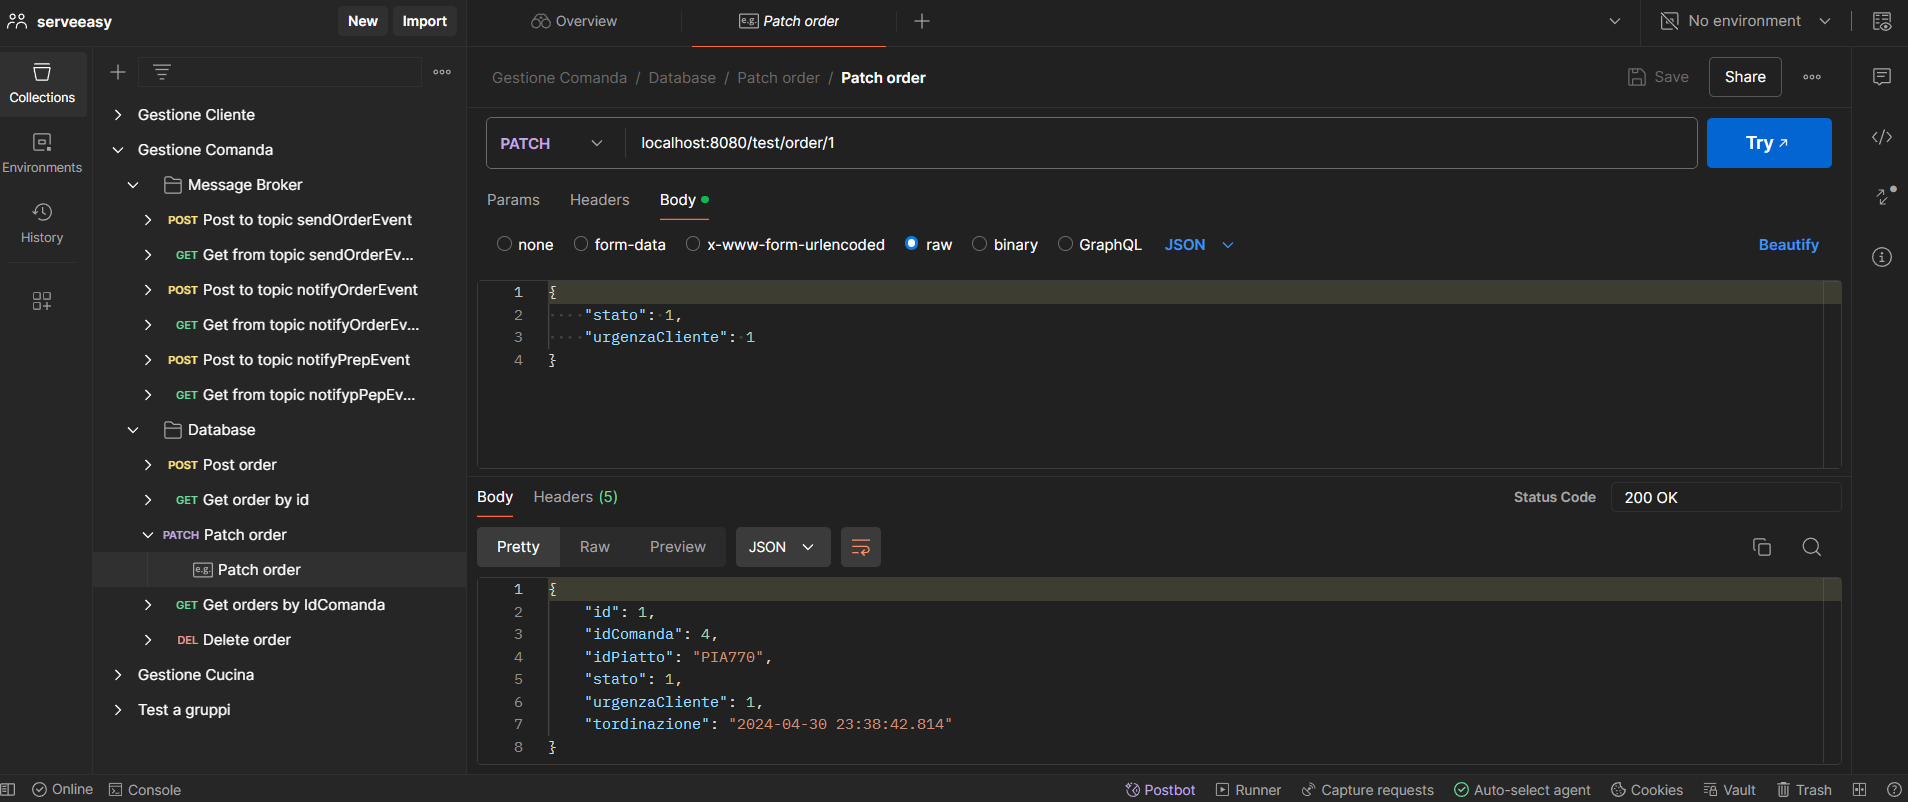
\includegraphics[width=1\linewidth]{iterazione1/images/postman-screen.png}
    \caption{Esempio applicativo Postman}
    \label{fig:postman-screen}
\end{figure}
In questo esempio viene effettuata una richiesta di PATCH di aggiornamento parziale di un ordine, viene specificata la variabile di percorso \textit{id=1} e il corpo della richiesta, ossia il JSON con il quale sono descritti i campi di \textit{stato} e \textit{urgenzaCliente} da aggiornare. Si può notare il codice di risposta 200 OK che viene restituito quando una richiesta HTTP è stata completata con successo e il corpo della risposta, ovvero un JSON contenente l'oggetto OrdineDTO serializzato.
\clearpage